\subsubsection{Backend Introduction}

The backend of the Ola compiler compiles IR into target assembly code. It takes the standard LLVM IR generated by the frontend as input and the Ola assembly code as output.

Its pipeline process is as follows figure \ref{fig:ola-lang-backend}:
\begin{figure}[!htbp]
    \centering
    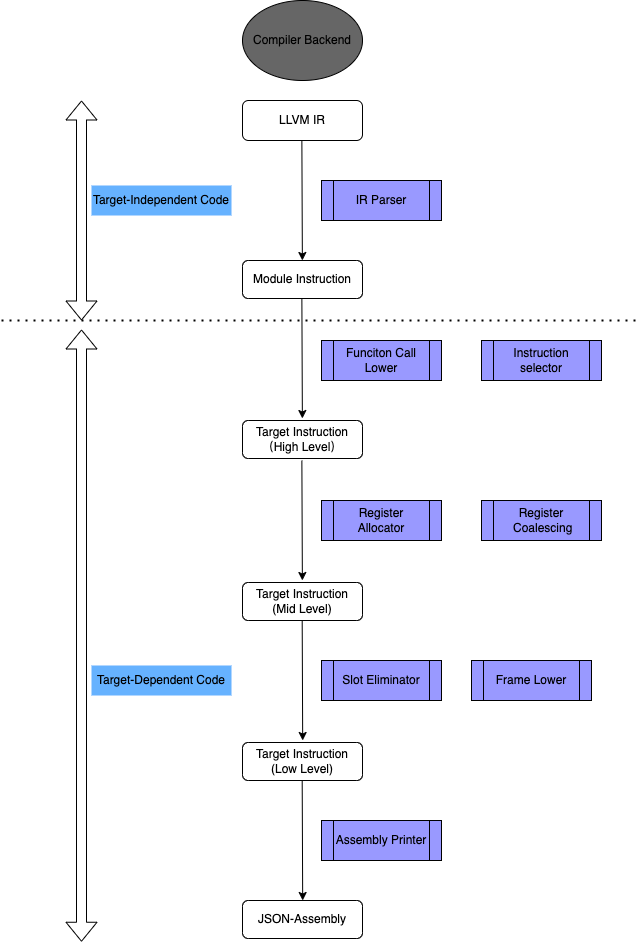
\includegraphics[width=0.6\textwidth]{ola-lang-backend.png}
    \caption{ola-lang backend pipeline}
    \label{fig:ola-lang-backend}
\end{figure}

An example ola-lang assembly code for computing sqrt of type u32 with prophet version is as follows:
\begin{lstlisting}[language={}]
{
  "program": "u32_sqrt:\n.LBL3_0:\n  mov r3 r1\n  mov r1 r3\n.PROPHET3_0:\n  mov r0 psp\n  mload r0 [r0,0]\n  range r0\n  mul r2 r0 r0\n  assert r2 r3\n  ret\nmain:\n.LBL4_0:\n  add r8 r8 4\n  mstore [r8,-2] r8\n  mov r1 4\n  call sqrt_test\n  add r8 r8 -4\n  end\nsqrt_test:\n.LBL5_0:\n  add r8 r8 6\n  mstore [r8,-2] r8\n  mov r0 r1\n  mstore [r8,-3] r0\n  mload r1 [r8,-3]\n  call u32_sqrt\n  mstore [r8,-4] r0\n  mload r0 [r8,-4]\n  add r8 r8 -6\n  ret\n",
  "prophets": [
    {
      "label": ".PROPHET3_0",
      "code": "%{\n    entry() {\n        cid.y = sqrt(cid.x);\n    }\n%}",
      "inputs": [
        "cid.x"
      ],
      "outputs": [
        "cid.y"
      ]
    }
  ]
}
\end{lstlisting}


The backend data structure contains mainly lists, module instructions, and target instructions.
The Application Binary Interface(ABI) then contains Function call specification and mapping relationships to virtual memory.

The backend codegen pipeline process is briefly as follows:
\begin{itemize}
    \item IR parsing

    \item Function call lowering

    \item Instruction selection

    \item Register allocation

    \item Slot elimination

    \item Stack frame handling

    \item Assembly printing
\end{itemize}
